\chapter{Introduction} \label{chap:intro}
The goal of this thesis is the implementation of a parallel implementation of a pointer analysis. As well as researching to what extent such an implementation presents advantages or disadvantages over other analyses that are not strictly parallel in nature.

\section{Structure of this Thesis}
This thesis is divided into three chapters.
The first chapter \autoref{chap:intro} lays the groundwork for the implementation and goes into detail what ideas were persued in order to develop the implementation. All related work and it's influences on this work is discussed here, as well as the motivation for the implementation itself. Furthermore the fundamentals of pointer analysis are explained here with code samples and an end to end analysis workflow that aims to illustrate the connection between actual code and its representation in a pointer analysis.

In the second chapter \autoref{chap:main} the software, namely PTAGPU, that was developed as part of this thesis, is described in detail. Design decisions, integrations with other software libraries and correctness are elaborated here.
The experimental benchmark results and how they wre generated are also presented here.

The last chapter \autoref{chap:conclusion} covers possible future work that could further improve the implementation and explore more ideas concerning parallel pointer analyses.
This chapter also discusses the experimental results from \autoref{chap:main}.


\subsubsection{Field-sensitivity}
field sensitivity is nice
\subsubsection{Flow-sensitivity}
flow sensitivity is nice
\subsubsection{Context-sensitivity}
Context sensitivity is nice
\subsubsection{Array-sensitivity}
array sensitivity is nice
\subsubsection{Structure-sensitivity}
Structure sensitivity is nice

field - flow - context - array sensitivity; structure sensitivity: \autocite{balatsouras2016structure}
\subsection{Steengards Analysis}
general idea
\subsection{Andersens Analysis}
inclusion based pta idea, timeframe
\subsection{Wave Propagation}
explain optimizations in modern sequential pta implementations: diffpts, worklists, consed hashes, \autocite{pereirawave}
\subsection{LLVM - Generating Data for Analysis}
what is llvm, general compiler architecture: front / backends, llvm-IR

go through instrs, and how they are relevant to pta, explain constraints \autocite{lin2015alias}
\section{Related Work}
\subsection{Context Free Languages}
first general idea: \autocite{reps1998program} first idea of gemm for cflpq \autocite{azimov2018context} kronecker product idea \autocite{orachev2020context} evaluation \autocite{mishin2019evaluation} spbla library \autocite{orachev2021spbla}, current draft [Taming Transitive Redundancy for Context-Free Language Reachability] fron SVF, parallel pta via cfl \autocite{su2014parallel}
\subsection{Sequential Analyses}
\subsubsection{SVF}
svf idea, built on top of llvm, \autocite{sui2016svf}, briefly explain all subcomponents i.e. memleak detection: \autocite{sui2014detecting} demand driven VF: \autocite{sui2018value} new alternative, faster, better results than svf \autocite{shi2018pinpoint}
\subsection{GPU Accelerated Analyses}
\subsubsection{Graspan}
original idea \autocite{zheng2008demand} big data approach on cpu \autocite{wang2017graspan} and gpu \autocite{zuo2021systemizing} alternative impl \autocite{gu2020towards} based on \autocite{mendez2012gpu} and \autocite{mendez2010parallel}
\section{Motivation}
general alias analysis is undecidable
\subsection{Static Analysis in Software Development}
finding bugs is becoming harder

inter procedural analysis scalability; create a single machine implementation that used parallel hardware and integrates into SVF


This is a citation \autocite{juliani2018unity}!
\begin{figure}
    \centering
    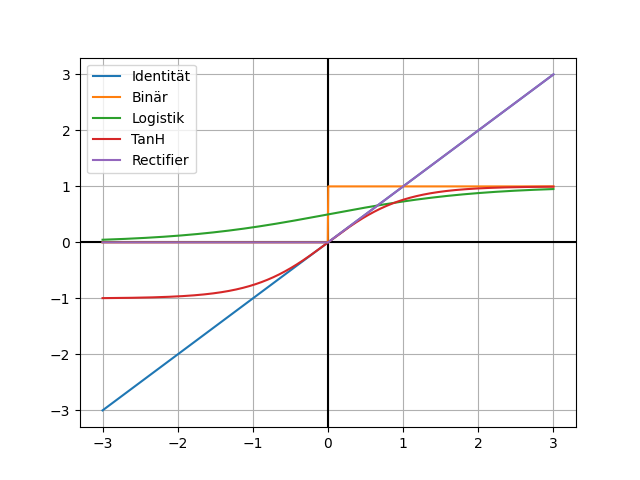
\includegraphics[width=0.8\textwidth]{img/test.png}
    \caption{Einige typische Aktivierungsfunktionen}
    \label{fig:actfn}
\end{figure}

\begin{figure}
    \centering
    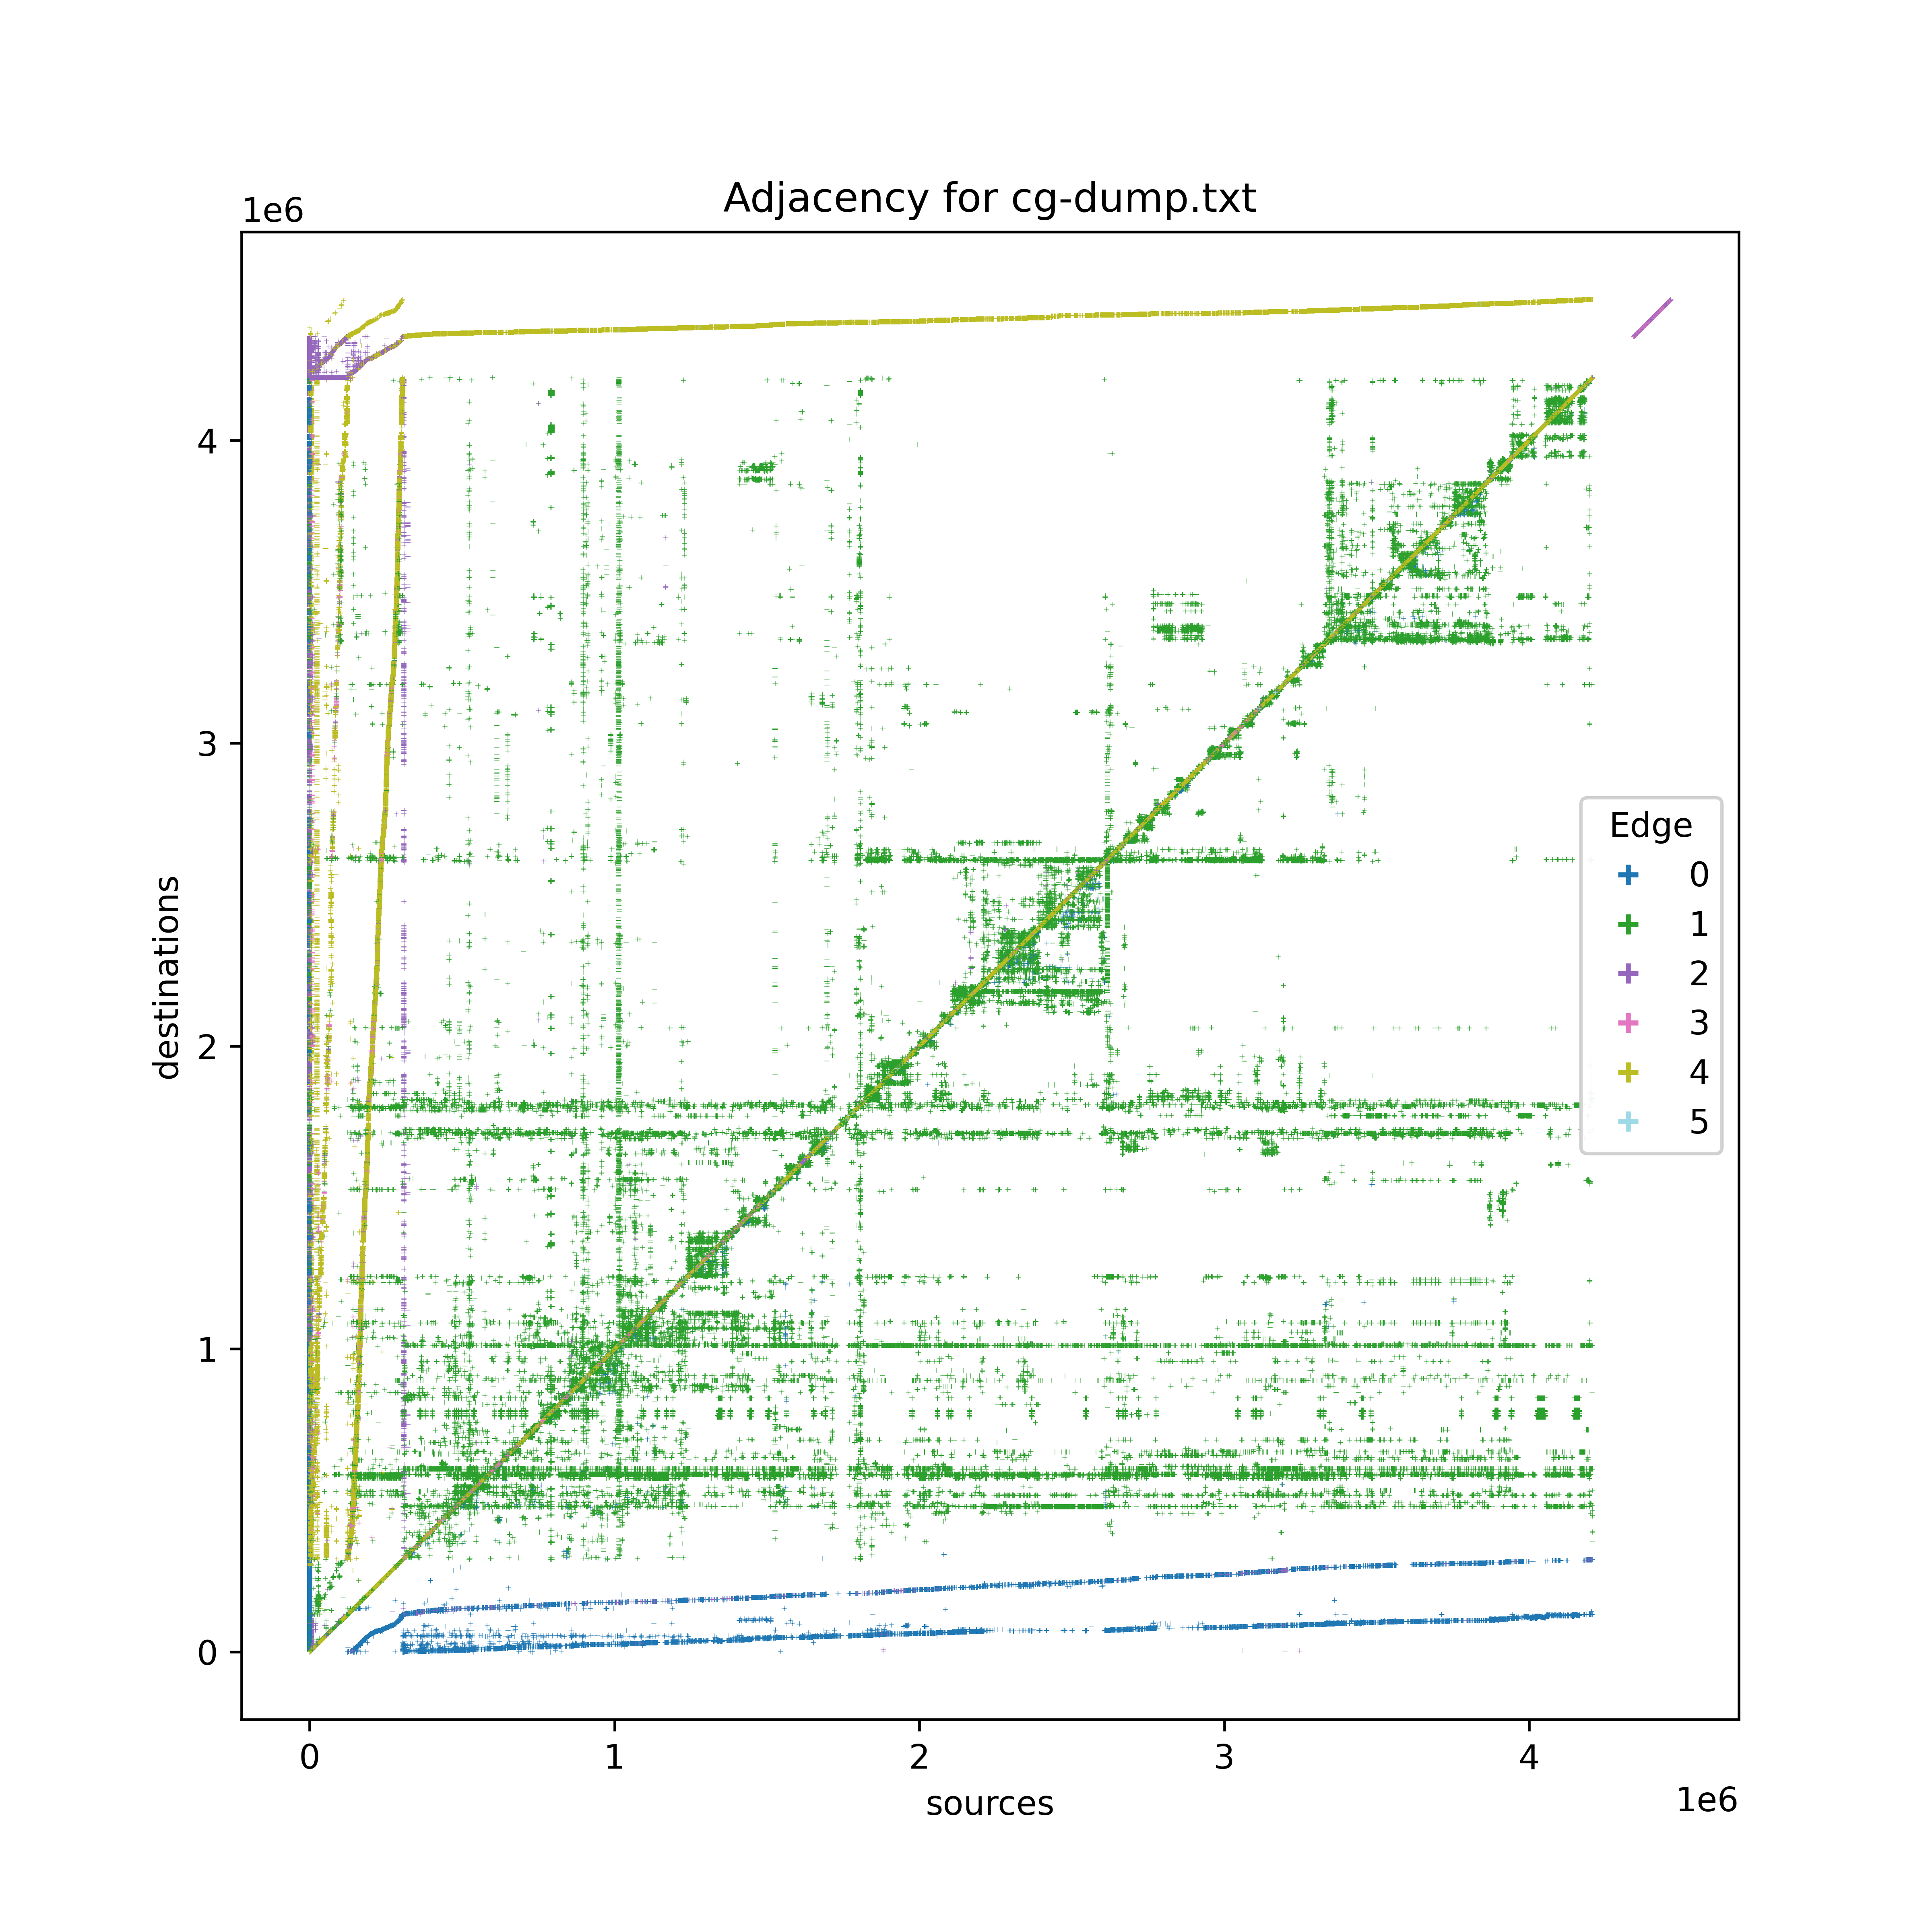
\includegraphics[width=1.\textwidth]{img/linux-consg.png}
    \caption{Adjacency Plot for the Constraint Graph of the Linux Kernel}
    \label{fig:linux-consg}
\end{figure}

\begin{minted}[mathescape, linenos]{python}

    # Note: $\pi=\lim_{n\to\infty}\frac{P_n}{d}$
    title = "Hello World"

    sum = 0
    for i in range(10):
     sum += i
\end{minted}



\begin{table}[h!]
    \begin{center}
        \caption{More rows.}
        \label{tab:table1}
        \begin{tabular}{l|S|r}
            \textbf{Value 1} & \textbf{Value 2} & \textbf{Value 3} \\
            $\alpha$         & $\beta$          & $\gamma$         \\
            \hline
            1                & 1110.1           & a                \\
            2                & 10.1             & b                \\
            3                & 23.113231        & c                \\
            4                & 25.113231        & d                \\ % <-- added row here
        \end{tabular}
    \end{center}
\end{table}